\documentclass[10pt,a4paper, polish]{article}
\usepackage[utf8]{inputenc}
\usepackage[T1]{fontenc}
\usepackage{amsmath}
\usepackage{amsfonts}
\usepackage{amssymb}
\usepackage{float}
\usepackage{graphicx}
\author{Jakub Jaśków}
\title{Obliczenia Naukowe - Lista nr 2}
\graphicspath{{plots/}}

\begin{document}
\maketitle
\section{Zad}
\subsection*{Opis}
Powtórzyć zadanie 5 z listy 1. Usunąć ostatnią 9 z $x_4$ i ostatnią 7 z $x_5$. Porównać i objaśnić wyniki.\\
$x = [2.718281828, -3.141592654, 1.414213562, 0.5772156649, 0.3010299957]$\\
$x' = [2.718281828, -3.141592654, 1.414213562, 0.577215664, 0.301029995]$\\
$y = [1486.2497, 878366.9879, -22.37492, 4773714.647, 0.000185049]$
\subsection*{Rozwiązanie}
Modyfikujemy kod z zadania 5 listy 1 tak aby wartości odpowiadały tym z polecenia.
\subsection*{Wyniki}
\begin{table}[H]
\centering
\caption{}
\begin{tabular}{|l|l|l|l|}
\hline
\textbf{Float32} & \textbf{Function} & \textbf{New} & \textbf{Old} \\
\hline
& forwards() & -0.4999443 & -0.4999443 \\
& backwards() & -0.4543457 & -0.4543457 \\
& maxToMax() & -0.5 & -0.5 \\
& revmaxToMax() & -0.5 & -0.5 \\
\hline
\textbf{Float64} & \textbf{Function} & \textbf{New} & \textbf{Old} \\
\hline
& forwards() & -0.004296342739891585 & 1.0251881368296672e-10 \\
& backwards() & -0.004296342998713953 & -1.5643308870494366e-10 \\
& maxToMax() & -0.004296342842280865 & 0.0 \\
& revmaxToMax() & -0.004296342842280865 & 0.0 \\
\hline
\end{tabular}
\end{table}

Jak widać wyniki algorytmów dla typu \textbf{Float32} są takie same. Nie jest to szokujące, ponieważ zmiany w danych zostały dokonane na końcach precyzji \textbf{Float32}.\\\\
Wyniki dla \textbf{Float64} różnią się jednak znacząco. Porównujące je do prawidłowej nowej wartości $sum(x',y) = -0.004296343192495245$ widzimy, że nowe wyniki nie tak bardzo różnią się od wartości prawidłowych. Różnica jest rzędu $10^-10$
\subsection*{Wnioski}
Zauważyć możemy, że o ile błąd bezwzględny dla obu danych wejściowych mają podobny rząd wielkości to wartości iloczynu znacząco się zmieniła, w wyniku czego błąd względny drastycznie zmalał. Wartość realna iloczynu skalarnego znacznie się zmieniła.\\\\
Na skutek wyżej wymienionych obserwacji możemy wywnioskować, że to nie wina dopasowania naszych algorytmów, ale uwarunkowanie zadania sprawia, że niewielkie zmiany danych wejściowych w znaczny sposób wpływają na wyniki.
\section{Zad}
\subsection*{Opis}
Narysować wykres funkcji $f(x)=e^{x}ln(1+e^{-x})$ w co najmniej dwóch programach do wizualizacji. Policzyć granicę funkcji przy $lim_{x\rightarrow\infty}f(x)$. Porównać wykres funkcji z jej granicą i wyjaśnić zjawisko.
\subsection*{Rozwiązanie}
Do rozwiązania tego zadania użyjemy 4 różnych programów graficzny: \textbf{Wolfram Alpha}, \textbf{Symbolab}, \textbf{Julia}, \textbf{Desmos}.
Wartości przedstawione na wykresach porównamy z limitem funkcji $lim_{x\rightarrow\infty}(e^{x}ln(1+e^{-x})) = 1$.
\subsection*{Wyniki}
\begin{figure}[H]
\caption{Desmos}
\centering
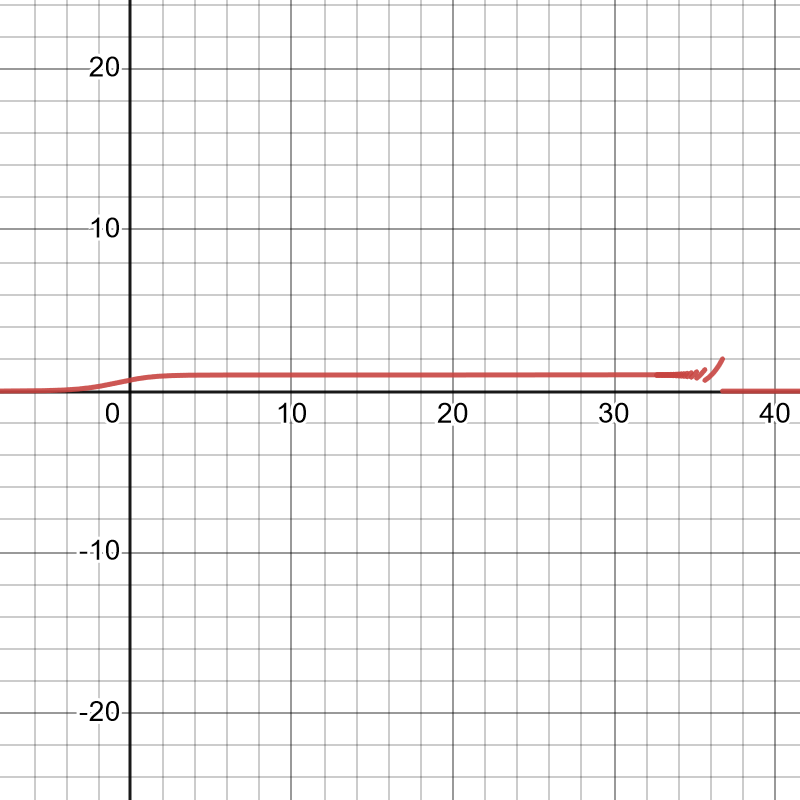
\includegraphics[scale=0.2]{plots/ex2/desmos.png}
\end{figure}
\begin{figure}[H]
\caption{Wolfram Alpha - przybliżenie}
\centering
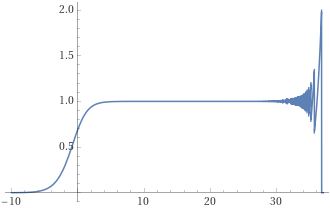
\includegraphics[scale=0.5]{plots/ex2/wolfram-alpha-closeup.png}
\end{figure}
\begin{figure}[H]
\caption{Julia - przybliżenie}
\centering
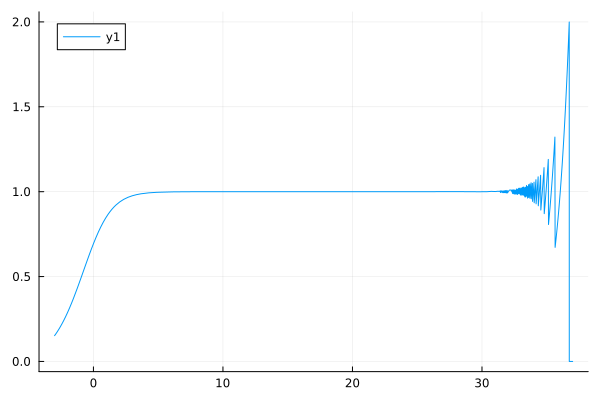
\includegraphics[scale=0.3]{plots/ex2/julia-closeup.png}
\end{figure}
\begin{figure}[H]
\caption{Symbolab - przybliżenie}
\centering
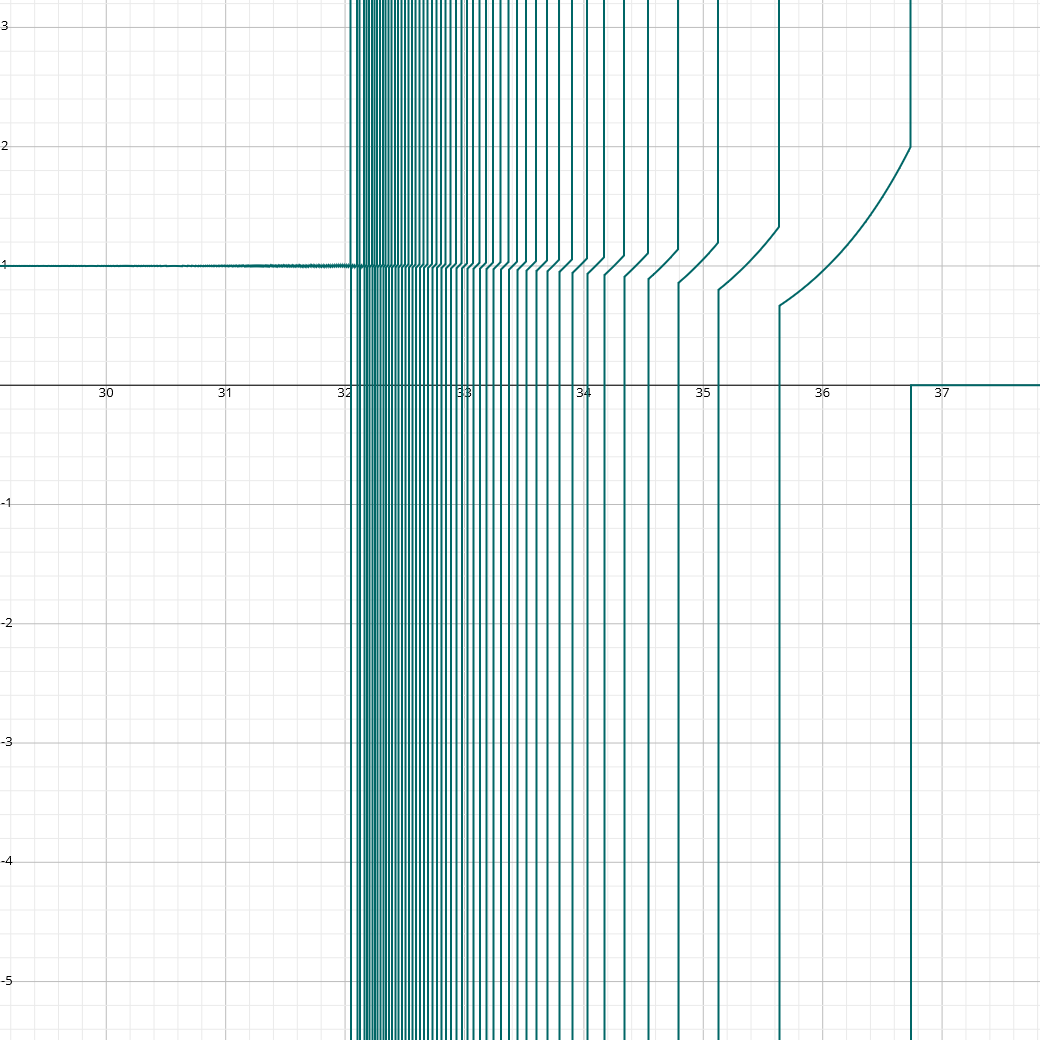
\includegraphics[scale=0.11]{plots/ex2/symbolab-closeup.png}
\end{figure}
Widać, że wykresy różnią się od prawdziwych wartości funkcji.
\subsection*{Wnioski}
Wartość granicy funkcji odczytana z wykresu znacząco różni się od tej wyliczonej ręcznie. Dzieje się tak ponieważ dla dużych $x$ wyrażenie w środku logarytmu $1+e^{-x} = 1+( \frac{1}{e^x})  \approx 1$, a $e^x*ln(1) = e^x*0=0$. Możemy zatem wnioskować, że zadanie to jest źle uwarunkowane, co potwierdzają aż 4 wykresy z odrębnych programów graficzno-matematycznych.
\section{Zad}
\subsection*{Opis}
Rozwiązać układ liniowy $ \textbf{Ax = b} $, gdzie $\textbf{A}$ to macierz współczynników $ \textbf{A} \in \mathbb{R}^{n \times n} $, a $ \textbf{b} \in \mathbb{R}^{n} $ to wektor prawych stron. Macierz $ \textbf{A} $ generujemy dzięki funkcjom \textbf{hilb(n)} $(n > 1)$ oraz \textbf{matcond(n, c)} $(n = 5, 10, 15; c = 1, 10, 10^3, 10^7, 10^{12}, 10^{16})$,  pobranym ze strony wykładowcy.\\\\
Prawidłowe rozwiązanie to wektor jedynek, czyli $ \textbf{x} = (1,..., 1)^\textit{T}$. Naszym zadaniem jest rozwiązać równanie  $ \textbf{Ax = b} $ za pomocą dwóch algorytmów: eliminacji Gaussa $(x=A\b) $ oraz $x = A^{-1}b$. Porównać policzony $\tilde{\textbf{x}}$ z $ \textbf{x} = (1,..., 1)^\textit{T}$, czyli \textbf{policzyć błędy względne}.
\subsection*{Rozwiązanie}
Wykonujemy wyżej wymienione algorytmy w pętli for i odczytujemy wyniki.
\subsection*{Wyniki}
\begin{table}[H]
\centering
\caption{$hilb(n)$}
\begin{tabular}{|c|p{3cm}|c|c|c|c|}
\hline
\textbf{n} & \textbf{cond(A)} & \textbf{rank(A)} & \textbf{Gauss Relative Error} & \textbf{Invert Relative Error} \\
\hline
\hline
1 & 1.0 & 1 & 0.0 & 0.0 \\
\hline
5 & 476607.2502425855 & 5 & $1.6828426299227195\times10^{-12}$ & $3.3544360584359632\times10^{-12}$ \\
\hline
9 & $4.9315375594102344\times10^{11}$ & 9 & $3.8751634185032475\times10^{-6}$ & $4.541268303176643\times10^{-6}$ \\
\hline
13 & $3.1883950689209334\times10^{18}$ & 11 & 0.11039701117868264 & 5.331275639426837 \\
\hline
17 & $1.249010044779401\times10^{18}$ & 12 & 13.707236683836307 & 10.516942378369349 \\
\hline
21 & $3.2902428208431683\times10^{18}$ & 13 & 44.089455838364245 & 34.52041154914292 \\
\hline
25 & $1.3309197502927598\times10^{18}$ & 13 & 7.095757204652332 & 21.04404299195525 \\
\hline
29 & $8.060274133463556\times10^{18}$ & 14 & 60.095450394724104 & 43.40383683199056 \\
\hline
33 & $1.1705237268888885\times10^{19}$ & 14 & 37.556822732776205 & 32.889697413799794 \\
\hline
37 & $5.871718859396612\times10^{18}$ & 15 & 13.974714130452178 & 16.39248770656996 \\
\hline
41 & $1.052376926308958\times10^{20}$ & 15 & 41.348771577098454 & 40.75749340255354 \\
\hline
45 & $1.1757348627810804\times10^{19}$ & 15 & 244.58124814685377 & 179.92316617880468 \\
\hline
49 & $6.145459250718421\times10^{18}$ & 16 & 24.15062009750964 & 35.92139018094681 \\
\hline
53 & $1.5742943175983743\times10^{19}$ & 16 & 845.0038584060173 & 744.7484527726867 \\
\hline
57 & $8.190646875595796\times10^{19}$ & 16 & 202.94297451029178 & 179.84690703784088 \\
\hline
61 & $9.02594600748171\times10^{18}$ & 16 & 70.48680315009305 & 67.11583016786831 \\
\hline
\end{tabular}
\end{table}

\begin{table}[H]
\centering
\caption{$matcond(n,c)$}
\begin{tabular}{|c|p{3.4cm}|p{1cm}|c|c|c|}
\hline
$\textbf{n}$ & $\textbf{cond}(A)$ & $\textbf{rank}(A)$ & \textbf{Gauss Relative Error} & \textbf{Invert Relative Error} & $\textbf{c}$ \\
\hline
5 & 1.0000000000000013 & 5 & $2.7194799110210365 \times 10^{-16}$ & $1.1102230246251565 \times 10^{-16}$ & $10^0$ \\
\hline
5 & 9.999999999999993 & 5 & $2.220446049250313 \times 10^{-16}$ & $2.808666774861361 \times 10^{-16}$ & $10^1$ \\
\hline
5 & 1000.000000000075 & 5 & $1.3331924943818472 \times 10^{-14}$ & $1.3197745560238665 \times 10^{-14}$ & $10^3$ \\
\hline
5 & 9.999999988554455e6 & 5 & $3.199232142364538 \times 10^{-10}$ & $1.4257906835893972 \times 10^{-10}$ & $10^7$ \\
\hline
5 & 1.0000033494643236e12 & 5 & $2.036498994500373 \times 10^{-5}$ & $1.8843214470258284 \times 10^{-5}$ & $10^{12}$ \\
\hline
5 & 6.688500865685893e15 & 4 & 0.5889024188140967 & 0.451559796704711 & $10^{16}$ \\
\hline
10 & 1.0000000000000007 & 10 & $1.6088660122137096 \times 10^{-16}$ & $3.3121136700345433 \times 10^{-16}$ & $10^0$ \\
\hline
10 & 9.999999999999993 & 10 & $3.8459253727671276 \times 10^{-16}$ & $5.301242283512285 \times 10^{-16}$ & $10^1$ \\
\hline
10 & 1000.0000000000341 & 10 & $1.5780952360285983 \times 10^{-14}$ & $2.0871838533448145 \times 10^{-14}$ & $10^3$ \\
\hline
10 & 1.0000000009265918e7 & 10 & $4.6003538792904206 \times 10^{-10}$ & $4.5321682416826476 \times 10^{-10}$ & $10^7$ \\
\hline
10 & 1.0000299226323792e12 & 10 & $5.088133827453193 \times 10^{-5}$ & $5.29604895008069 \times 10^{-5}$ & $10^{12}$ \\
\hline
10 & 3.722163178554466e16 & 9 & 0.20999773729554208 & 0.23783898505606685 & $10^{16}$ \\
\hline
20 & 1.0000000000000013 & 20 & $4.3920512659784095 \times 10^{-16}$ & $3.8218127502839273 \times 10^{-16}$ & $10^0$ \\
\hline
20 & 10.0 & 20 & $3.979805003092567 \times 10^{-16}$ & $4.2711132545550575 \times 10^{-16}$ & $10^1$ \\
\hline
20 & 1000.00000000008 & 20 & $2.3048828947687884 \times 10^{-15}$ & $1.3048309088140642 \times 10^{-14}$ & $10^3$ \\
\hline
20 & 1.0000000003904887e7 & 20 & $2.302074075751533 \times 10^{-10}$ & $2.4959292115882135 \times 10^{-10}$ & $10^7$ \\
\hline
20 & 9.999831732131125e11 & 20 & $4.404089447858288 \times 10^{-5}$ & $4.344454948384514 \times 10^{-5}$ & $10^{12}$ \\
\hline
20 & 9.624512830246104e15 & 19 & 0.04769860428854183 & 0.10502383733558494 & $10^{16}$ \\
\hline
\end{tabular}
\end{table}
\subsection*{Wnioski}

Znając wskaźnik uwarunkowania macierzy oraz błąd reprezentacji wektora prawych stron jesteśmy w stanie oszacować błąd względny naszej metody pomiarowej.\\\\
Błędy względne wyliczone na podstawie obu metod są znaczące. Nawet małych rozmiarów macierz Hilberta posiada bardzo duży wskaźnik uwarunkowania. Rozwiązywanie równań liniowych na macierzy Hilberta metodą Gaussa zdaje się być nieco dokładniejsze niż metoda odwrotnej macierzy.\\\\
W przypadku macierzy losowych o ustalonym wskaźniku uwarunkowania ciężko stwierdzić, czy któryś algorytm jest lepszy. Dla każdej macierzy błędy względne obu algorytmów są tego samego rzędu.\\\\
Skoro algorytmy działają w odpowiedni sposób dla macierzy losowych, oznacza to, że podpunkt w którym współczynniki równania określa macierz Hilberta jest zadaniem źle uwarunkowanym.
\section{Zad}
\subsection*{A}
\subsubsection*{Opis}
Naszym zadaniem jest zbadanie złośliwego wielomianu Wilkinsona:
$$ \prod_{i=1}^{20}(x-i) $$\\
Sprawdź jak pakiet \textbf{Polynomials} języka Julia radzi sobie z wyznaczaniem pierwiastków wielomianu. Sprawdź czy wartości zwrócone przez pakiet faktycznie są pierwiastkami tego wielomianu.\\
\subsubsection*{Rozwiązanie}
Wczytujemy współczynniki z pliku dostępnego na stronie wykładowcy. Używamy pakietu Polynomials do znalezienia pierwiastków wielomianu oraz sprawdzamy, czy faktycznie zerują wielomian.\\
\subsubsection*{Wyniki}
\begin{table}[H]
\center
\caption{Pierwiastki wielomianu, wartości wielomianów}
\begin{tabular}{|c|p{3cm}|p{3.4cm}|p{3.4cm}|p{3.5cm}|}
\hline
$k$ & $z_k$ & $|P(z_k)|$ & $|p(z_k)|$ & $|z_k - k|$ \\
\hline
1 & 0.9999999999996989 & 35696.50964788257 & 5.518479490350445e6 & 3.0109248427834245e-13 \\
\hline
2 & 2.0000000000283182 & 176252.60026668405 & 7.37869762990174e19 & 2.8318236644508943e-11 \\
\hline
3 & 2.9999999995920965 & 279157.6968824087 & 3.3204139316875795e20 & 4.0790348876384996e-10 \\
\hline
4 & 3.9999999837375317 & 3.0271092988991085e6 & 8.854437035384718e20 & 1.626246826091915e-8 \\
\hline
5 & 5.000000665769791 & 2.2917473756567076e7 & 1.8446752056545688e21 & 6.657697912970661e-7 \\
\hline
6 & 5.999989245824773 & 1.2902417284205095e8 & 3.320394888870117e21 & 1.0754175226779239e-5 \\
\hline
7 & 7.000102002793008 & 4.805112754602064e8 & 5.423593016891273e21 & 0.00010200279300764947 \\
\hline
8 & 7.999355829607762 & 1.6379520218961136e9 & 8.262050140110275e21 & 0.0006441703922384079 \\
\hline
9 & 9.002915294362053 & 4.877071372550003e9 & 1.196559421646277e22 & 0.002915294362052734 \\
\hline
10 & 9.990413042481725 & 1.3638638195458128e10 & 1.655260133520688e22 & 0.009586957518274986 \\
\hline
11 & 11.025022932909318 & 3.585631295130865e10 & 2.24783329792479e22 & 0.025022932909317674 \\
\hline
12 & 11.953283253846857 & 7.533332360358197e10 & 2.886944688412679e22 & 0.04671674615314281 \\
\hline
13 & 13.07431403244734 & 1.9605988124330817e11 & 3.807325552826988e22 & 0.07431403244734014 \\
\hline
14 & 13.914755591802127 & 3.5751347823104315e11 & 4.612719853150334e22 & 0.08524440819787316 \\
\hline
15 & 15.075493799699476 & 8.21627123645597e11 & 5.901011420218566e22 & 0.07549379969947623 \\
\hline
16 & 15.946286716607972 & 1.5514978880494067e12 & 7.010874106897764e22 & 0.05371328339202819 \\
\hline
17 & 17.025427146237412 & 3.694735918486229e12 & 8.568905825736165e22 & 0.025427146237412046 \\
\hline
18 & 17.99092135271648 & 7.650109016515867e12 & 1.0144799361044434e23 & 0.009078647283519814 \\
\hline
19 & 19.00190981829944 & 1.1435273749721195e13 & 1.1990376202371257e23 & 0.0019098182994383706 \\
\hline
20 & 19.999809291236637 & 2.7924106393680727e13 & 1.4019117414318134e23 & 0.00019070876336257925 \\
\hline
\end{tabular}
\end{table}

\begin{table}[H]
\centering
\caption{Faktyczne pierwiastki wielomianu}
\begin{tabular}{|c|c|c|}
\hline
$k$ & $|P(k)|$ & $|p(k)|$ \\
\hline
1 & $0.0$ & $0$ \\
\hline
2 & $8192.0$ & $0$ \\
\hline
3 & $27648.0$ & $0$ \\
\hline
4 & $622592.0$ & $0$ \\
\hline
5 & $2.176e6$ & $0$ \\
\hline
6 & $8.84736e6$ & $0$ \\
\hline
7 & $2.4410624e7$ & $0$ \\
\hline
8 & $5.89824e7$ & $0$ \\
\hline
9 & $1.45753344e8$ & $0$ \\
\hline
10 & $2.27328e8$ & $0$ \\
\hline
11 & $4.79074816e8$ & $0$ \\
\hline
12 & $8.75003904e8$ & $0$ \\
\hline
13 & $1.483133184e9$ & $0$ \\
\hline
14 & $2.457219072e9$ & $0$ \\
\hline
15 & $3.905712e9$ & $0$ \\
\hline
16 & $6.029312e9$ & $0$ \\
\hline
17 & $9.116641408e9$ & $0$ \\
\hline
18 & $1.333988352e10$ & $0$ \\
\hline
19 & $1.9213101568e10$ & $0$ \\
\hline
20 & $2.7193344e10$ & $0$ \\
\hline
\end{tabular}
\end{table}
\subsubsection*{Wnioski}
Jak widać na zamieszczonej powyżej tabeli 4 wyznaczone przez nas pierwiastki nie są dokładne. \\\\
Dlaczego tak się dzieje? Na ratunek przybywam nam tabela 5, na której widać, że prawdziwe pierwiastki wielomianu $P(x)$ nie zerują go. Dzieje się tak, ponieważ wartości współczynników przechowywane są w arytmetyce Float64. Dla małych współczynników tego wielomianu oznacza to pozbycie się kilku cyfr znaczących.\\\\
Na tabeli 4 można też zaobserwować mniemaną "złośliwość" tego wielomianu. Pomimo bardzo małych odchyleń $|z_k-k|$ uzyskane przez nas wartości wielomianu Wilkinsona postaci $P(z_k)$ oraz $p(z_k)$ są \textbf{ogromne}.\\\\
Możemy zatem wnioskować, że zadanie to jest źle uwarunkowane.
\subsection*{B}
\subsubsection*{Opis}
Powtórzyć eksperyment \textbf{Wilkinsona} - minimalnie zaburzyć wielomian oraz wyjaśnić zjawisko.
\subsubsection*{Rozwiązanie}
To samo co w podpunkcie A) powtarzamy dla podpunktu B). Zmieniamy tylko współczynnik $-210$ na $-210-2^{-23}$.
\subsubsection*{Wyniki}
\begin{table}[H]
\centering
\caption{Wartości wielomianu dla $p[2] = -210-2^{-23}$}
\begin{tabular}{|p{0.1cm}|p{3.2cm}|p{3.2cm}|p{3.2cm}|p{3.2cm}|}
\hline
$k$ & $z_k$ & $|P(z_k)|$ & $|p(z_k)|$ & $|z_k - k|$ \\
\hline
1 & $0.9999999999998357 + 0.0\text{im}$ & $20259.872313418207$ & $3.0131001276845885\times 10^6$ & $1.6431300764452317\times 10^{-13}$ \\
\hline
2 & $2.0000000000550373 + 0.0\text{im}$ & $346541.4137593836$ & $7.37869763029606\times 10^{19}$ & $5.503730804434781\times 10^{-11}$ \\
\hline
3 & $2.99999999660342 + 0.0\text{im}$ & $2.3655796995492927\times 10^{6}$ & $3.320413920110016\times 10^{20}$ & $3.3965799062229962\times 10^{-9}$ \\
\hline
4 & $4.000000089724362 + 0.0\text{im}$ & $1.0018343680854071\times 10^{7}$ & $8.854437817429642\times 10^{20}$ & $8.972436216225788\times 10^{-8}$ \\
\hline
5 & $4.99999857388791 + 0.0\text{im}$ & $4.6254074679189965\times 10^{7}$ & $1.844672697408419\times 10^{21}$ & $1.4261120897529622\times 10^{-6}$ \\
\hline
6 & $6.000020476673031 + 0.0\text{im}$ & $2.0241763473292372\times 10^{8}$ & $3.320450195282313\times 10^{21}$ & $2.0476673030955794\times 10^{-5}$ \\
\hline
7 & $6.99960207042242 + 0.0\text{im}$ & $1.710626634091394\times 10^{9}$ & $5.422366528916004\times 10^{21}$ & $0.00039792957757978087$ \\
\hline
8 & $8.007772029099446 + 0.0\text{im}$ & $1.869950954754733\times 10^{10}$ & $8.289399860984408\times 10^{21}$ & $0.007772029099445632$ \\
\hline
9 & $8.915816367932559 + 0.0\text{im}$ & $1.3757318900886914\times 10^{11}$ & $1.160747250177049\times 10^{22}$ & $0.0841836320674414$ \\
\hline
10 & $10.095455630535774 - 0.6449328236240688\text{im}$ & $1.491101451791542\times 10^{12}$ & $1.7212892853670706\times 10^{22}$ & $0.6519586830380407$ \\
\hline
11 & $10.095455630535774 + 0.6449328236240688\text{im}$ & $1.491101451791542\times 10^{12}$ & $1.7212892853670706\times 10^{22}$ & $1.1109180272716561$ \\
\hline
12 & $11.793890586174369 - 1.6524771364075785\text{im}$ & $3.2967412333942234\times 10^{13}$ & $2.8568401004080956\times 10^{22}$ & $1.665281290598479$ \\
\hline
13 & $11.793890586174369 + 1.6524771364075785\text{im}$ & $3.2967412333942234\times 10^{13}$ & $2.8568401004080956\times 10^{22}$ & $2.0458202766784277$ \\
\hline
14 & $13.992406684487216 - 2.5188244257108443\text{im}$ & $9.545851019861934\times 10^{14}$ & $4.934647147686795\times 10^{22}$ & $2.518835871190904$ \\
\hline
15 & $13.992406684487216 + 2.5188244257108443\text{im}$ & $9.545851019861934\times 10^{14}$ & $4.934647147686795\times 10^{22}$ & $2.7128805312847097$ \\
\hline
16 & $16.73074487979267 - 2.812624896721978\text{im}$ & $2.7421389712291324\times 10^{16}$ & $8.484694713563005\times 10^{22}$ & $2.9060018735375106$ \\
\hline
17 & $16.73074487979267 + 2.812624896721978\text{im}$ & $2.7421389712291324\times 10^{16}$ & $8.484694713563005\times 10^{22}$ & $2.825483521349608$ \\
\hline
18 & $19.5024423688181 - 1.940331978642903\text{im}$ & $4.252503605694188\times 10^{17}$ & $1.3181947820607215\times 10^{23}$ & $2.4540214463129764$ \\
\hline
19 & $19.5024423688181 + 1.940331978642903\text{im}$ & $4.252503605694188\times 10^{17}$ & $1.3181947820607215\times 10^{23}$ & $2.0043294443099486$ \\
\hline
20 & $20.84691021519479 + 0.0\text{im}$ & $1.3743593159265196\times 10^{18}$ & $1.5911084081430876\times 10^{23}$ & $0.8469102151947894$ \\
\hline
\end{tabular}
\end{table}
\subsubsection*{Wnioski}
Wartości przedstawione na tabeli 6 potwierdzają wnioski o złym uwarunkowaniu zadanie z podpunktu A. Marginalne zaburzenie jednego z współczynników wielomianu powoduje pojawienie się rozwiązań zespolonych. Zauważalny jest też wzrost wartości wynikowych wielomianów $P(z_k)$, $p(z_k)$ oraz $|z_k - k|$.
\section{Zad}
\subsection*{Opis}
Wyznaczyć 40 pierwszych wyrazów ciągu:
$$ p_{n+1} := p_n + rp_n(1-p_n)\text{, dla }n = 0,1,...$$, gdzie $r = 3$ a $p_0 = 0.01$.\\
Sposoby wyznaczania ciągu:\\
1. Arytmetyka Float32\\
2. Arytmetyka Float32 z obcięciem $p_{10}$ do 3 cyfr po przecinku $(p_{10} = 0.722)$\\
3. Arytmetyka Float64
\subsection*{Rozwiązanie}
Ustawiamy odpowiednie parametry a następnie wykonujemy 10 iteracji pętli \textbf{for}. Kiedy wyjdziemy z pierwszej pętli tworzymy nową zmienną, która będzie reprezentowała $p_{10}=0.722$. Znowu wchodzimy do pętli i wykonujemy następne 30 iteracji. Wszystkie wartości wyświetlamy na bieżąco w terminalu w sposób ułatwiający nam konwersję do tabeli.
\subsection*{Wyniki}
\begin{table}[H]
\centering
\caption{Zad 5.1 i Zad5.2}
\begin{tabular}{|c|c|c|c|}
\hline
$n$ & Float32 & Float32 z obcięciem & Float64 \\
\hline
0 & 0.01 & 0.01 & 0.01 \\
\hline
1 & 0.0397 & 0.0397 & 0.0397 \\
\hline
2 & 0.15407173 & 0.15407173 & 0.15407173000000002 \\
\hline
3 & 0.5450726 & 0.5450726 & 0.5450726260444213 \\
\hline
4 & 1.2889781 & 1.2889781 & 1.2889780011888006 \\
\hline
5 & 0.1715188 & 0.1715188 & 0.17151914210917552 \\
\hline
6 & 0.5978191 & 0.5978191 & 0.5978201201070994 \\
\hline
7 & 1.3191134 & 1.3191134 & 1.3191137924137974 \\
\hline
8 & 0.056273222 & 0.056273222 & 0.056271577646256565 \\
\hline
9 & 0.21559286 & 0.21559286 & 0.21558683923263022 \\
\hline
10 & 0.7229306 & 0.722 & 0.722914301179573 \\
\hline
11 & 1.3238364 & 1.3241479 & 1.3238419441684408 \\
\hline
12 & 0.037716985 & 0.036488414 & 0.03769529725473175 \\
\hline
13 & 0.14660022 & 0.14195944 & 0.14651838271355924 \\
\hline
14 & 0.521926 & 0.50738037 & 0.521670621435246 \\
\hline
15 & 1.2704837 & 1.2572169 & 1.2702617739350768 \\
\hline
16 & 0.2395482 & 0.28708452 & 0.24035217277824272 \\
\hline
17 & 0.7860428 & 0.9010855 & 0.7881011902353041 \\
\hline
18 & 1.2905813 & 1.1684768 & 1.2890943027903075 \\
\hline
19 & 0.16552472 & 0.577893 & 0.17108484670194324 \\
\hline
20 & 0.5799036 & 1.3096911 & 0.5965293124946907 \\
\hline
21 & 1.3107498 & 0.09289217 & 1.3185755879825978 \\
\hline
22 & 0.088804245 & 0.34568182 & 0.058377608259430724 \\
\hline
23 & 0.3315584 & 1.0242395 & 0.22328659759944824 \\
\hline
24 & 0.9964407 & 0.94975823 & 0.7435756763951792 \\
\hline
25 & 1.0070806 & 1.0929108 & 1.315588346001072 \\
\hline
26 & 0.9856885 & 0.7882812 & 0.07003529560277899 \\
\hline
27 & 1.0280086 & 1.2889631 & 0.26542635452061003 \\
\hline
28 & 0.9416294 & 0.17157483 & 0.8503519690601384 \\
\hline
29 & 1.1065198 & 0.59798557 & 1.2321124623871897 \\
\hline
30 & 0.7529209 & 1.3191822 & 0.37414648963928676 \\
\hline
31 & 1.3110139 & 0.05600393 & 1.0766291714289444 \\
\hline
32 & 0.0877831 & 0.21460639 & 0.8291255674004515 \\
\hline
33 & 0.3280148 & 0.7202578 & 1.2541546500504441 \\
\hline
34 & 0.9892781 & 1.3247173 & 0.29790694147232066 \\
\hline
35 & 1.021099 & 0.034241438 & 0.9253821285571046 \\
\hline
36 & 0.95646656 & 0.13344833 & 1.1325322626697856 \\
\hline
37 & 1.0813814 & 0.48036796 & 0.6822410727153098 \\
\hline
38 & 0.81736827 & 1.2292118 & 1.3326056469620293 \\
\hline
39 & 1.2652004 & 0.3839622 & 0.0029091569028512065 \\
\hline
40 & 0.25860548 & 1.093568 & 0.011611238029748606 \\
\hline
\end{tabular}
\end{table}
\subsection*{Wnioski}
Na tabeli 7 możemy zaobserwować, że początkowe wartości wyrazów ciągu są bardzo podobne. Dopiero dla $n = 19$ uwidacznia się znaczna różnica w wartości Float32 z obcięciem, a dla $n = 22$ także dla samej wartości Float32. Oddalenie się od siebie wartości spowodowane jest postępującą akumulacja błędów, którą zawdzięczamy miedzy innymi potęgowaniu ukrytemu we wzorze ciągu.\\\\
Możemy zatem wnioskować, że wyznaczanie kolejnych wyrazów ciągu $p_n$ jest procesem niestabilnym, ponieważ z każdą iteracją błędy nakładają się na siebie, potęgując rozstrzał pomiędzy wartościami oczekiwanymi a rzeczywistymi.\\\\
Nawet wartości $p_n$ wyliczone w arytmetyce Float64 dla odpowiedni dużego $n$ staną się \textbf{BARDZO} oddalone od rzeczywistości.
\section{Zad}
\subsection*{Opis}
Rozważmy ciągi rekurencyjne wyrażone wzorem:
$$x_{n+1} = x_n^2 + c$$
Naszym zadaniem jest przeprowadzenie obserwacji zachowania ciągu, gdy $c = -2 \wedge x_0 \in \{1, 2, 1.99999999999999\}$ oraz $c = -1 \wedge x_0 \in \{1, 0.75, 0.25, -1\}$.
\subsection*{Rozwiązanie}
Aby uzyskać rozwiązania wystarczy przeprowadzić 40 iteracji wyrażenia $$x_{n+1} = x_n^2 + c$$ dla danych wejściowych podanych wyżej oraz na bieżąco wyświetlać potrzebne nam wyniki w terminalu.
\subsection*{Wyniki}
\begin{table}[H]
\centering
\caption{Wartości $x_n$ dla $c = -2$}
\begin{tabular}{|c|c|c|c|}
\hline
$n$ & $x_0=1$ & $x_0=2$ & $x_0=1.99999999999999$ \\
\hline
1 & -1.0 & 2.0 & 1.99999999999996 \\
\hline
2 & -1.0 & 2.0 & 1.9999999999998401 \\
\hline
3 & -1.0 & 2.0 & 1.9999999999993605 \\
\hline
4 & -1.0 & 2.0 & 1.999999999997442 \\
\hline
5 & -1.0 & 2.0 & 1.9999999999897682 \\
\hline
6 & -1.0 & 2.0 & 1.9999999999590727 \\
\hline
7 & -1.0 & 2.0 & 1.999999999836291 \\
\hline
8 & -1.0 & 2.0 & 1.9999999993451638 \\
\hline
9 & -1.0 & 2.0 & 1.9999999973806553 \\
\hline
10 & -1.0 & 2.0 & 1.999999989522621 \\
\hline
11 & -1.0 & 2.0 & 1.9999999580904841 \\
\hline
12 & -1.0 & 2.0 & 1.9999998323619383 \\
\hline
13 & -1.0 & 2.0 & 1.9999993294477814 \\
\hline
14 & -1.0 & 2.0 & 1.9999973177915749 \\
\hline
15 & -1.0 & 2.0 & 1.9999892711734937 \\
\hline
16 & -1.0 & 2.0 & 1.9999570848090826 \\
\hline
17 & -1.0 & 2.0 & 1.999828341078044 \\
\hline
18 & -1.0 & 2.0 & 1.9993133937789613 \\
\hline
19 & -1.0 & 2.0 & 1.9972540465439481 \\
\hline
20 & -1.0 & 2.0 & 1.9890237264361752 \\
\hline
21 & -1.0 & 2.0 & 1.9562153843260486 \\
\hline
22 & -1.0 & 2.0 & 1.82677862987391 \\
\hline
23 & -1.0 & 2.0 & 1.3371201625639997 \\
\hline
24 & -1.0 & 2.0 & -0.21210967086482313 \\
\hline
25 & -1.0 & 2.0 & -1.9550094875256163 \\
\hline
26 & -1.0 & 2.0 & 1.822062096315173 \\
\hline
27 & -1.0 & 2.0 & 1.319910282828443 \\
\hline
28 & -1.0 & 2.0 & -0.2578368452837396 \\
\hline
29 & -1.0 & 2.0 & -1.9335201612141288 \\
\hline
30 & -1.0 & 2.0 & 1.7385002138215109 \\
\hline
31 & -1.0 & 2.0 & 1.0223829934574389 \\
\hline
32 & -1.0 & 2.0 & -0.9547330146890065 \\
\hline
33 & -1.0 & 2.0 & -1.0884848706628412 \\
\hline
34 & -1.0 & 2.0 & -0.8152006863380978 \\
\hline
35 & -1.0 & 2.0 & -1.3354478409938944 \\
\hline
36 & -1.0 & 2.0 & -0.21657906398474625 \\
\hline
37 & -1.0 & 2.0 & -1.953093509043491 \\
\hline
38 & -1.0 & 2.0 & 1.8145742550678174 \\
\hline
39 & -1.0 & 2.0 & 1.2926797271549244 \\
\hline
40 & -1.0 & 2.0 & -0.3289791230026702 \\
\hline
\end{tabular}
\end{table}

Dla parametrów $c = -2$ i $x_0 \in {1,2}$ ciąg ten jest bardzo stabilny. Z każdą iteracja otrzymamy tą samą wartość. Natomiast dla $x_0 = 1.99999999999999$, czyli bardzo małego odchylenia, po $n = 22$ uzyskane przez nas wyniki są chaotyczne. 

\begin{table}[H]
\centering
\caption{Wartości $x_n$ dla $c = -1$}
\begin{tabular}{|c|c|c|c|c|}
\hline
$n$ & $x_0=1$ & $x_0=-1$ & $x_0=0.75$ & $x_0=0.25$ \\
\hline
1 & 0.0 & 0.0 & -0.4375 & -0.9375 \\
\hline
2 & -1.0 & -1.0 & -0.80859375 & -0.12109375 \\
\hline
3 & 0.0 & 0.0 & -0.3461761474609375 & -0.9853363037109375 \\
\hline
4 & -1.0 & -1.0 & -0.8801620749291033 & -0.029112368589267135 \\
\hline
5 & 0.0 & 0.0 & -0.2253147218564956 & -0.9991524699951226 \\
\hline
6 & -1.0 & -1.0 & -0.9492332761147301 & -0.0016943417026455965 \\
\hline
7 & 0.0 & 0.0 & -0.0989561875164966 & -0.9999971292061947 \\
\hline
8 & -1.0 & -1.0 & -0.9902076729521999 & -5.741579369278327e-6 \\
\hline
9 & 0.0 & 0.0 & -0.01948876442658909 & -0.9999999999670343 \\
\hline
10 & -1.0 & -1.0 & -0.999620188061125 & -6.593148249578462e-11 \\
\hline
11 & 0.0 & 0.0 & -0.0007594796206411569 & -1.0 \\
\hline
12 & -1.0 & -1.0 & -0.9999994231907058 & 0.0 \\
\hline
13 & 0.0 & 0.0 & -1.1536182557003727e-6 & -1.0 \\
\hline
14 & -1.0 & -1.0 & -0.9999999999986692 & 0.0 \\
\hline
15 & 0.0 & 0.0 & -2.6616486792363503e-12 & -1.0 \\
\hline
16 & -1.0 & -1.0 & -1.0 & 0.0 \\
\hline
17 & 0.0 & 0.0 & 0.0 & -1.0 \\
\hline
18 & -1.0 & -1.0 & -1.0 & 0.0 \\
\hline
19 & 0.0 & 0.0 & 0.0 & -1.0 \\
\hline
20 & -1.0 & -1.0 & -1.0 & 0.0 \\
\hline
21 & 0.0 & 0.0 & 0.0 & -1.0 \\
\hline
22 & -1.0 & -1.0 & -1.0 & 0.0 \\
\hline
23 & 0.0 & 0.0 & 0.0 & -1.0 \\
\hline
24 & -1.0 & -1.0 & -1.0 & 0.0 \\
\hline
25 & 0.0 & 0.0 & 0.0 & -1.0 \\
\hline
26 & -1.0 & -1.0 & -1.0 & 0.0 \\
\hline
27 & 0.0 & 0.0 & 0.0 & -1.0 \\
\hline
28 & -1.0 & -1.0 & -1.0 & 0.0 \\
\hline
29 & 0.0 & 0.0 & 0.0 & -1.0 \\
\hline
30 & -1.0 & -1.0 & -1.0 & 0.0 \\
\hline
31 & 0.0 & 0.0 & 0.0 & -1.0 \\
\hline
32 & -1.0 & -1.0 & -1.0 & 0.0 \\
\hline
33 & 0.0 & 0.0 & 0.0 & -1.0 \\
\hline
34 & -1.0 & -1.0 & -1.0 & 0.0 \\
\hline
35 & 0.0 & 0.0 & 0.0 & -1.0 \\
\hline
36 & -1.0 & -1.0 & -1.0 & 0.0 \\
\hline
37 & 0.0 & 0.0 & 0.0 & -1.0 \\
\hline
38 & -1.0 & -1.0 & -1.0 & 0.0 \\
\hline
39 & 0.0 & 0.0 & 0.0 & -1.0 \\
\hline
40 & -1.0 & -1.0 & -1.0 & 0.0 \\
\hline
\end{tabular}
\end{table}
Jeżeli radykalnie zmienimy równanie naszego ciągu i zastąpimy $c = -2$ na $c = -1$ to uzyskamy podobne zachowanie. Dla $x_0 \in \{-1, 1\}$ wartości oscylują pomiędzy $0$ a $-1$, dla $x_0 \in \{-0.75, 0.25\}$ na początku otrzymujemy zachowanie chaotyczne, które po paru iteracjach stabilizuje się pomiędzy $0$ a $-1$.
\subsection*{Wnioski}
Wyznaczanie kolejnych wyrazów ciągów rekurencyjnych może mieć różną stabilność w zależności od parametrów wejściowych. Przykładem tego jest nasz ciąg $x_{n+1} = x_n^2 + c$. Wynika z tego, że pomimo obecności potęgi w naszym wzorze istnieje klasa zadań/problemów które "stabilizują" się; błędy akumulacyjne są w nich pomijane. Pozwala nam to na wykonywanie niektórych obliczeń na maszynach o skończonej precyzji.\\\\
Dlaczego więc wartości dla $c=-2$ i $x_0=1.99999999999999$ zachowują się tak chaotycznie? Ponieważ zadanie to jest źle uwarunkowane dla dobranych danych wejściowych. Odejmujemy liczby bliskie sobie a następnie akumulujemy błąd poprzez podnoszenie do kwadratu.
\end{document}